% !TEX program = pdflatex
% Square One Chess --- front matter (cover to lists), ISI Kef style
% Overleaf: pdfLaTeX. Compile TWICE so the table of contents updates.
% Upload logo-uj.png and logo-isik.png.
% =============================================================================
\documentclass[12pt,a4paper,oneside]{report}

\usepackage{iftex}
\ifPDFTeX
  \usepackage[T1]{fontenc}
  \usepackage[utf8]{inputenc}
  \usepackage{fix-cm}
  \usepackage{mathptmx}
\else
  \usepackage{fontspec}
  \setmainfont{Times New Roman}
\fi

\usepackage[a4paper,left=2.5cm,right=2.5cm,top=2.2cm,bottom=2.2cm]{geometry}
\usepackage{scrextend}
\changefontsizes[19.5pt]{16pt}
\usepackage{graphicx}
\graphicspath{{logos/}{./logos/}{./}}
\usepackage{setspace}
\usepackage[table]{xcolor}
\usepackage[explicit]{titlesec}
\usepackage{fancyhdr}
\usepackage{truncate}
\usepackage[titles]{tocloft}
\usepackage{float}
\usepackage[section]{placeins}
\usepackage[skip=6pt,font=small,labelfont=bf,justification=centering]{caption}
\usepackage{booktabs}
\usepackage{array}
\usepackage{tabularx}
\usepackage{longtable}
\usepackage{enumitem}
\usepackage{etoolbox}
\usepackage{tikz}
\usetikzlibrary{positioning,arrows.meta}
\usepackage{hyperref}
\usepackage{pdfpages}

% Colours sampled from the FitZone PFE PDF
\definecolor{chapterblue}{RGB}{31,72,124}     % chapter titles (Chapitre 1)
\definecolor{sectionblue}{RGB}{0,111,192}     % section titles (1.1, 1.2)
\definecolor{subsectionblue}{RGB}{68,113,196} % subsection titles (1.2.2)
\definecolor{plantumlbg}{RGB}{132,85,84}
\definecolor{toclink}{RGB}{0,0,127}

\hypersetup{colorlinks=true,linkcolor=toclink,urlcolor=toclink}

\setcounter{tocdepth}{3}
\setcounter{secnumdepth}{3}

\setstretch{1.22}
\setlength{\parindent}{0pt}
\setlength{\parskip}{0.45em}

\newcommand{\StudentName}{Lasmer Dhia Eddin}
\newcommand{\IndustrySupervisor}{M. Aziz Thraya}
\newcommand{\AcademicSupervisor}{Dr. Hmida Hmida}

\renewcommand{\chaptername}{Chapter}

\titleformat{\chapter}[display]
  {\normalfont\color{chapterblue}\bfseries}
  {\huge\chaptername~\thechapter}
  {10pt}
  {\huge #1}
\titleformat{name=\chapter,numberless}[display]
  {\normalfont\color{chapterblue}\bfseries}
  {}
  {0pt}
  {\huge #1}
\titlespacing*{\chapter}{0pt}{16pt}{22pt}

\titleformat{\section}
  {\normalfont\LARGE\bfseries\color{sectionblue}}
  {\thesection}{0.8em}{#1}
\titleformat{\subsection}
  {\normalfont\Large\bfseries\color{subsectionblue}}
  {\thesubsection}{0.8em}{#1}

\renewcommand{\chaptermark}[1]{\markboth{\chaptername~\thechapter}{}}
\pagestyle{fancy}
\fancyhf{}
\fancyhead[L]{\footnotesize\nouppercase{\truncate{0.58\headwidth}{\leftmark}}}
\fancyhead[R]{\footnotesize Square One PFE 2025--2026}
\fancyfoot[C]{\thepage}
\renewcommand{\headrulewidth}{0.4pt}
\setlength{\headheight}{16pt}

\renewcommand{\contentsname}{Table of Contents}
\renewcommand{\listfigurename}{List of Figures}
\renewcommand{\listtablename}{List of Tables}
\renewcommand{\cftchappresnum}{Chapter~}
\renewcommand{\cftchapaftersnum}{\hspace{0.7em}}
\renewcommand{\cftchapfont}{\bfseries\color{chapterblue}}
\renewcommand{\cftchappagefont}{\bfseries\color{chapterblue}}
\renewcommand{\cftsecfont}{\color{sectionblue}}
\renewcommand{\cftsecpagefont}{\color{sectionblue}}
\renewcommand{\cftsubsecfont}{\color{subsectionblue}}
\renewcommand{\cftsubsecpagefont}{\color{subsectionblue}}
\setlength{\cftchapnumwidth}{10.4em}
\cftsetindents{chapter}{0em}{10.4em}
\cftsetindents{section}{1.4em}{2.8em}
\cftsetindents{subsection}{4.2em}{3.4em}
\renewcommand{\cftchapdotsep}{\cftdotsep}
\setlength{\cftbeforechapskip}{10pt}
\setlength{\cftbeforesecskip}{2pt}
\setlength{\cftbeforesubsecskip}{1pt}

% Tables stay on the page: smaller type, no float queue after figures.
\AtBeginEnvironment{table}{%
  \FloatBarrier
  \footnotesize
  \setstretch{1.05}%
  \setlength{\tabcolsep}{3.2pt}%
  \setlist[itemize]{leftmargin=1em,itemsep=1pt,topsep=2pt,parsep=0pt,partopsep=0pt}%
}
\AtBeginEnvironment{longtable}{%
  \footnotesize
  \setstretch{1.05}%
  \setlength{\tabcolsep}{3.2pt}%
}

\newcommand{\includelogo}[1]{%
  \IfFileExists{#1}{%
    \includegraphics[height=2.35cm,keepaspectratio]{#1}%
  }{%
    \fbox{\begin{minipage}[c][2.1cm][c]{2.1cm}\centering\tiny Upload\\[2pt] #1\end{minipage}}%
  }%
}

\newcommand{\figbox}[1]{%
  \begin{figure}[H]
    \centering
    \fbox{\parbox{0.88\linewidth}{\centering\vspace{1.6cm}\textit{[#1]}\vspace{1.6cm}}}
    \caption{#1}
  \end{figure}%
}

\newcommand{\umlfig}[2]{%
\begin{figure}[H]
\centering
\IfFileExists{#1}{%
  \includegraphics[width=0.92\linewidth,height=0.34\textheight,keepaspectratio]{#1}%
}{\fbox{\parbox{0.92\linewidth}{\centering\vspace{1.4cm}\textit{[Upload #1]}\vspace{1.4cm}}}}
\caption{#2}
\end{figure}%
}

\newcommand{\uishot}[2]{%
\begin{figure}[H]
\centering
\IfFileExists{#1}{%
  \includegraphics[width=0.88\linewidth,height=0.32\textheight,keepaspectratio]{#1}%
}{\fbox{\parbox{0.92\linewidth}{\centering\vspace{1.6cm}\textit{[Screenshot: upload #1]}\vspace{1.6cm}}}}
\caption{#2}
\end{figure}%
}

% #1 logo file, #2 title, #3 description, #4 web key, #5 webography number
\newcommand{\techfig}[5]{%
\noindent\textbf{#2.} #3\par
\vspace{0.35em}
\begin{figure}[H]
\centering
\IfFileExists{#1}{%
  \includegraphics[height=2.2cm,keepaspectratio]{#1}%
}{\IfFileExists{logos/#1}{%
  \includegraphics[height=2.2cm,keepaspectratio]{logos/#1}%
}{\fbox{\parbox[c][2.0cm][c]{2.2cm}{\centering\tiny Upload #1}}}}
\caption{#2}
\label{fig:tech-#4}
\end{figure}%
}

% #1 title, #2 description, #3 web key, #4 webography number
\newcommand{\techfigdraw}[4]{%
\noindent\textbf{#1.} #2\par
\vspace{0.35em}
\begin{figure}[H]
\centering
\begin{tikzpicture}
  \fill[rounded corners=5pt, plantumlbg] (0,0) rectangle (2.0,2.0);
  \node[white, font=\bfseries, align=center] at (1.0,1.0) {UML};
\end{tikzpicture}
\caption{#1}
\label{fig:tech-#3}
\end{figure}%
}

% Webography line: clickable n. jumps to the matching technology figure.
% #1 number, #2 key, #3 title, #4 url, #5 consulted date
\newcommand{\webitem}[5]{%
\item[{\hyperref[fig:tech-#2]{\textbf{#1.}}}]
  #3. \url{#4}. Consulted on #5.%
}

\newcommand{\tabbox}[2]{%
  \begin{table}[H]
    \centering
    \caption{#1}
    \begin{tabular}{p{0.28\linewidth}p{0.58\linewidth}}
      \toprule
      \textbf{Item} & \textbf{Description} \\
      \midrule
      #2
      \bottomrule
    \end{tabular}
  \end{table}%
}

\begin{document}

% ========================= PAGE 1: official ISI cover PDF =========================

\includepdf[pages=1,fitpaper,pagecommand={\thispagestyle{empty}}]{cover-isi.pdf}
% Cover is unnumbered. Authorization is page 1 of the body (FitZone style).
\setcounter{page}{1}

% ========================= PAGE 2: signed authorization (NCIS) =========================

\includepdf[pages=1,fitpaper,pagecommand={\thispagestyle{empty}}]{autorisation-ncis.pdf}
\clearpage
\normalsize

% ========================= PAGE 3: ACKNOWLEDGEMENTS =========================
\chapter*{Acknowledgements}
\addcontentsline{toc}{chapter}{Acknowledgements}
\thispagestyle{plain}

First of all, I would like to express my sincere gratitude to all of my teachers for their guidance and for the knowledge they have shared with me. Their expertise and availability have greatly helped me deepen my understanding and develop my skills.

I thank in particular \textbf{Dr. Hmida Hmida}, my academic supervisor. His patience, advice and constant encouragement have been a real support throughout this project. His involvement and kindness have been a genuine source of motivation.

I also wish to express my deep appreciation to \textbf{M. Aziz Thraya}, my industry supervisor. Thanks to him, I had the opportunity to join a dynamic and competent development team at \textbf{NCIS}. Every exchange with its members was enriching and broadened my perspective. Their support, creativity and willingness to share their experience contributed greatly to the success of this project.

% ========================= PAGE 3: DEDICATION =========================
\chapter*{Dedication}
\addcontentsline{toc}{chapter}{Dedication}
\thispagestyle{plain}

I dedicate this work and this project to all the people who have marked my path throughout this journey.

To \textbf{my mother}, \textbf{my father} and \textbf{my brother}, for their unconditional love, their support and their endless patience during all the years that led to this moment. Their trust in me and their encouragement in times of doubt have been the solid foundation of my motivation. Without their constant support, none of this would have been possible.

To my family, for their encouragement and kindness throughout my studies.

To my classmates \textbf{Aziz} and \textbf{Mohamed}, who were present throughout this academic path and brightened these years with their presence and sincere friendship.

To my friends \textbf{Amine} and \textbf{Ala}, who have been there from the first steps of this adventure and have accompanied every stage with solidarity and friendship.

\vspace{1.8cm}
\hfill \StudentName

% ========================= TOC (own page) / LOF / LOT =========================
\clearpage
\tableofcontents
\clearpage
\phantomsection
\addcontentsline{toc}{chapter}{List of Figures}
\listoffigures
\clearpage
\phantomsection
\addcontentsline{toc}{chapter}{List of Tables}
\listoftables
\clearpage

\chapter*{General Introduction}
\addcontentsline{toc}{chapter}{General Introduction}

In an environment marked by rapid technological change and continuous digital transformation, organisations seek to modernise their information systems in order to improve efficiency, optimise internal processes and offer more reliable services to their users. Digitalisation has become an essential lever: it supports better data management, the automation of repetitive tasks and a global improvement of the user experience.

The world of chess has followed the same movement. Online play now attracts a growing number of amateurs and competitive players who expect, on a single platform, live games with a clock, a fair pairing system, a traceable history of their matches, a social space and training tools that help them progress. When these needs are covered only by scattered websites, club notebooks or informal messaging groups, several difficulties appear: results are poorly recorded, games cannot be replayed easily, ratings remain unreliable, and there is no centralised, secure view of the activity of the community.

It is in this context that this final-year project was carried out at \textbf{NCIS}, a company specialised in the design and development of information-system and web solutions. The organisation supports its clients throughout the conception and implementation of modern digital applications adapted to their business needs, and it provided the professional setting of this internship.

The main objective of the project is to design and develop a real-time online chess web platform named \textbf{Square One}. The application aims to make it easier for players to create an account, play live games, join matchmaking, consult their history and replay finished games, while also offering a community layer (friends and chat), structured competitions (tournaments), training features (puzzles, play against the engine, AI game review) and a supervision space for the administrator. In this way, Square One automates the organisation of play and improves the interaction between the different actors of the system, namely the visitor, the player and the administrator.

The adopted architecture relies on a clear separation between the presentation layer, developed with \textbf{Angular 17}, and the business layer based on \textbf{Node.js / Express} with TypeScript. Data persistence is handled with \textbf{Prisma} and \textbf{SQLite}. Real-time communication uses \textbf{Socket.io}, chess rules are applied with \textbf{chess.js}, and training or analysis features rely on the \textbf{Stockfish} engine. This architecture favours the maintainability, the security and the scalability of the system.

The present report is structured as follows:
\begin{itemize}[leftmargin=1.4em,itemsep=0.45em,topsep=0.6em]
  \item The first chapter presents the general framework of the project, in particular the host organisation NCIS, the study of the existing situation, the proposed solution, as well as the methodologies and technologies used.
  \item The second chapter is devoted to the analysis and specification of the functional and non-functional requirements, the use-case diagrams and the product backlog.
  \item The third chapter details Release~1: access management and the account process (Sprints 1 and 2).
  \item The fourth chapter presents Release~2: live play, matchmaking, history and replay (Sprints 3 and 4).
  \item The fifth chapter describes Release~3: community, tournaments, training and supervision of the platform (Sprints 5, 6, 7 and 8).
  \item A general conclusion closes the report by presenting the results obtained, the limits of the work and the perspectives for improvement.
\end{itemize}

% Skeleton chapters so the TOC matches a full PFE (like the FitZone report)
\chapter{Project Framework}
\section{Introduction}
In this first chapter, we begin by presenting the host organisation where this final-year project takes place. We then study the existing situation and its limitations, in order to propose our solution. Finally, we present the working method as well as the tools used to carry out the project.

\section{Presentation of the host organisation}
\textbf{NCIS} is a Tunisian company specialised in information-technology services and in the development of web, mobile and desktop solutions. Thanks to a team of qualified professionals, the company supports its clients in the design and implementation of digital applications adapted to their business needs. Its activity goes well beyond simple programming: it covers the analysis of requirements, the construction of information systems and the follow-up of projects until delivery.

The development service accompanies the conception and the creation of tailor-made applications. From the planning phase to implementation, NCIS aims to deliver projects with a high level of quality, efficiency and performance. It is within this professional environment, under the supervision of \textbf{M. Aziz Thraya}, that the Square One Chess platform was designed and developed.

\begin{figure}[H]
\centering
\IfFileExists{logo-ncis.jpg}{%
  
\includegraphics[height=3.4cm,keepaspectratio]{logo-ncis.jpg}%
}{\IfFileExists{logo-ncis.png}{%
  \includegraphics[height=3.4cm,keepaspectratio]{logo-ncis.png}%
}{%
  \fbox{\parbox{0.55\linewidth}{\centering\vspace{1.4cm}\textit{[Upload logo-ncis.jpg]}\vspace{1.4cm}}}%
}}
\caption{Logo of NCIS}
\end{figure}

\subsection{Status and missions of the host organisation}
\textbf{NCIS} (\textit{Network and Computer Integration Services}) is a Tunisian limited company created in 2010--2011 and based in Tunis. It specialises in network and computer integration, system and network administration, VoIP, Wi-Fi infrastructures and the study of open-source or proprietary solutions adapted to the needs of its clients. Under the direction of \textbf{M. Aziz Thraya}, General Manager, the company also accompanies the design of digital applications. Its missions are to advise, design, implement and maintain reliable IT solutions, and to train its teams in a professional working environment.

\subsection{Development cycle}
The realisation of a project at NCIS follows a structured development cycle, from the expression of the need to the delivery of the solution:
\begin{itemize}[leftmargin=1.4em,itemsep=0.45em]
  \item \textbf{Planning:} this step consists in defining and organising the tasks to be carried out, estimating the workload associated with each of them, establishing a provisional schedule and identifying the resources required to reach the objectives. In the case of Square One, this planning was organised into releases and sprints.
  \item \textbf{Implementation and follow-up:} the validated features are implemented according to a structured process. Each item of the backlog passes through several statuses (to do, in progress, tested, done), with regular reviews with the industry supervisor.
  \item \textbf{Validation:} validation is the final evaluation of a feature. It makes it possible to obtain the official agreement needed to integrate the modifications into the platform (functional tests of the API, of the Angular interface and of real-time play).
  \item \textbf{Delivery:} once the modifications have been carried out, validated and accepted, the last step is to deliver an updated and usable version of the application (local deployment of the backend, of the database and of the web client).
\end{itemize}

\subsection{Organisational chart of NCIS}
The host organisation is a small structure centred on general management and a technical team. The internship was carried out under the authority of the General Manager, within the development / integration team.

\begin{figure}[H]
\centering
\begin{tikzpicture}[
  node distance=7mm and 4mm,
  box/.style={draw, rounded corners=2pt, align=center, inner sep=7pt, font=\small, minimum width=5.2cm}
]
  \node[box] (gm) {\textbf{M. Aziz Thraya}\\General Manager};
  \node[box, below=of gm] (team) {Technical team\\network, systems and development};
  \node[box, below=of team] (intern) {Internship --- Square One Chess\\\StudentName};
  \draw[-{Stealth}] (gm) -- (team);
  \draw[-{Stealth}] (team) -- (intern);
\end{tikzpicture}
\caption{Organisational chart of NCIS}
\end{figure}

\subsection{Internship location}
The internship takes place on the premises of NCIS, located at \textbf{07, rue 8805, Cit\'e El Khadra, 1003 Tunis}. This professional setting offers an environment that is favourable to learning, collaboration and the practical application of the knowledge acquired during the academic training at ISI Kef. The company is headquartered in Tunis, Tunisia, which is also where the internship was carried out.

\subsection{Previously completed IT projects}
NCIS has solid experience in information technology, covering network integration, system administration, VoIP, Wi-Fi infrastructures and the study of open-source or proprietary solutions. The company has designed and deployed various projects that answer the specific needs of its clients. These realisations illustrate its commitment to offering reliable, scalable and practical digital services, and they provided a professional context in which a complete web application such as Square One could be specified, developed and tested.

\begin{table}[H]
\centering
\caption{Examples of IT projects and services carried out by NCIS}
\label{tab:ncis-projects}
\begin{tabularx}{0.92\linewidth}{lX}
\toprule
\textbf{Domain} & \textbf{Typical realisations} \\
\midrule
Network integration & Cisco SMB and Ubiquiti UniFi infrastructures, VDI cabling, hotspot and Wi-Fi coverage \\
Systems and security & System and network administration, IT security consulting \\
VoIP & IP telephony solutions adapted to the client's organisation \\
Open-source / software & Study and adaptation of open-source or proprietary tools to business needs \\
\bottomrule
\end{tabularx}
\end{table}

\section{Study of the existing situation}
\subsection{Description of the existing situation}
Before the design of Square One, amateur and competitive chess practice was spread over several unconnected channels. Many players use general-purpose websites to play a game, messaging groups to organise a match, and paper notebooks or spreadsheets in a club to record results. Training (puzzles, engine analysis, game review) is often done on yet another service, when it is done at all.

There is therefore no single, coherent information system that follows the player from the creation of an account to live play, history, community, tournaments and training. Pairing is frequently informal, ratings are not always updated in a reliable way, finished games cannot always be replayed, and the administrator of a small community has no dashboard to supervise activity, reports or the health of the platform.

\subsection{Critique of the existing situation}
The existing situation presents several limitations:
\begin{itemize}[leftmargin=1.4em,itemsep=0.35em]
  \item The absence of a centralised application makes it difficult to follow live games, ratings and results in real time.
  \item Matchmaking and time control are not guaranteed when games are organised only by chat or inside a physical club.
  \item Game history is incomplete: many games are lost, and replay or PGN export is not always available.
  \item Social features (friends, presence, chat) are separated from the board, which weakens the community.
  \item Training tools (puzzles, play versus the engine, AI review) are not integrated with the player's own games.
  \item Tournaments, when they exist, are managed by hand, with a high risk of errors in the bracket.
  \item Security (authentication, sessions, roles) and administration (analytics, moderation) are not clearly defined for a small dedicated platform.
\end{itemize}

\begin{figure}[H]
\centering
\begin{tikzpicture}[
  box/.style={draw, rounded corners=2pt, align=center, inner sep=8pt, font=\small, text width=3.5cm, minimum height=2.1cm}
]
  \node[box] (a) {Club notebooks\\and spreadsheets};
  \node[box, right=8mm of a] (b) {Scattered websites\\and chat groups};
  \node[box, right=8mm of b] (c) {Training tools\\disconnected from play};
\end{tikzpicture}
\caption{Typical organisation of amateur chess practice before Square One}
\label{fig:existing-chess}
\end{figure}

\subsection{Proposed solution}
In order to overcome the limits identified above, we propose the design and development of a modern real-time web platform dedicated to online chess: \textbf{Square One}. The main objectives of the solution are:
\begin{itemize}[leftmargin=1.4em,itemsep=0.35em]
  \item To set up a secure authentication system according to the role of the user (Visitor, Player, Administrator).
  \item To provide an intuitive, ergonomic and responsive web interface (Angular~17).
  \item To allow live games with a clock, legal moves (\texttt{chess.js}) and real-time communication (Socket.io).
  \item To offer automatic matchmaking, a complete game history and a replay mode.
  \item To integrate a community layer (friends, presence, chat).
  \item To support structured competitions through tournaments and brackets.
  \item To provide training features: puzzles, play against Stockfish, and AI game review.
  \item To expose statistics, an Elo rating and a leaderboard.
  \item To give the administrator a supervision space (analytics of users and games).
\end{itemize}

\section{Methodologies and working environment}
\subsection{Project management methodology}
The Agile methodology is a project-management approach based on short and iterative development cycles, called sprints. Among the different Agile methods, we have chosen the \textbf{Scrum} framework.

Scrum is used to manage complex software projects. It relies on well-defined roles (Product Owner, Scrum Master, Development Team), regular events (sprints, reviews) and artefacts such as the product backlog.

\paragraph{Scrum principles.}
Scrum is based on three principles:
\begin{itemize}[leftmargin=1.4em,itemsep=0.35em]
  \item \textbf{Transparency:} all relevant information about the project is shared with the team.
  \item \textbf{Inspection:} frequent checks are carried out to evaluate the progress of the work.
  \item \textbf{Adaptation:} adjustments are applied quickly when the observed results move away from the objectives.
\end{itemize}

\paragraph{Key roles in Scrum.}
The project team is organised around three main roles:
\begin{itemize}[leftmargin=1.4em,itemsep=0.35em]
  \item \textbf{Scrum Master:} guarantees the correct application of the Scrum process. In this project, the role is assumed by \textbf{M. Aziz Thraya}.
  \item \textbf{Product Owner:} responsible for the link between the needs of the product and the development team. For Square One, the Product Owner is also \textbf{M. Aziz Thraya}.
  \item \textbf{Development team:} designs, develops and delivers the features of the product. In our case, this role is fulfilled by ourselves (\StudentName).
\end{itemize}

\paragraph{Use of UML.}
In this project we used the Unified Modeling Language (UML) in order to obtain a clear, structured and standardised design of the system. Three types of diagrams are used:
\begin{itemize}[leftmargin=1.4em,itemsep=0.35em]
  \item The \textbf{use-case diagram}, to identify the functional needs and to model the interactions between the actors and the system.
  \item The \textbf{sequence diagram}, to model the chronological flow of the business scenarios.
  \item The \textbf{class diagram}, to represent the static structure of the system (users, games, moves, tournaments, etc.).
\end{itemize}
The diagrams are produced with \textbf{PlantUML} and will be presented in the following chapters.

\begin{figure}[H]
\centering
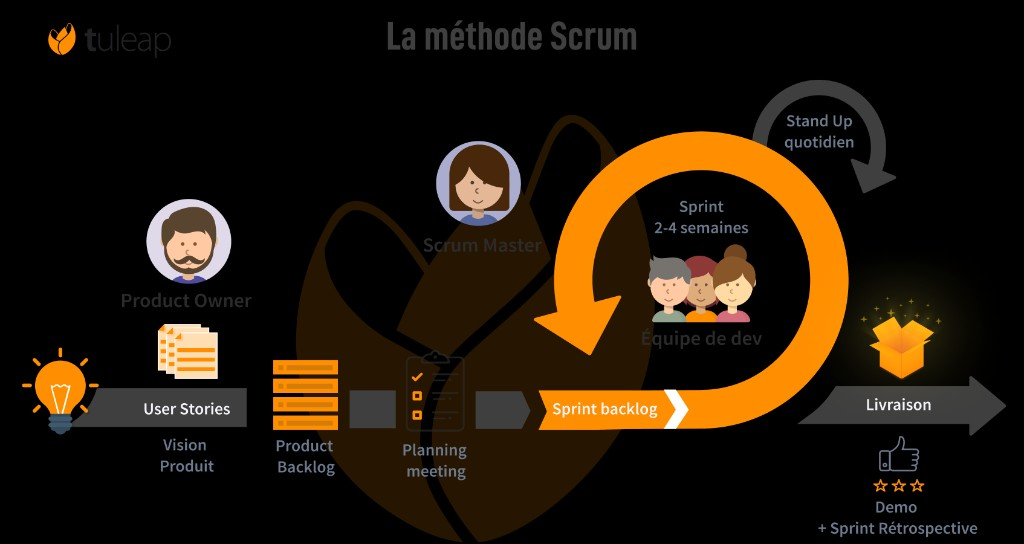
\includegraphics[width=0.92\linewidth,height=0.34\textheight,keepaspectratio]{fig-scrum.png}
\caption{The Scrum method}
\label{fig:scrum}
\end{figure}

\subsection{Software environment}
\paragraph{Front-end.}
The front-end development concerns the creation of the user interface, that is the visible and interactive part of the application. It includes the layout, the visual style and the dynamic elements displayed on the screen.

\techfig{angular.png}{Angular 17}{Open-source web framework used to build a single-page application based on standalone components, routing and reactive forms. It is the presentation layer of Square One.}{angular}{1}

\techfig{html5.png}{HTML5}{Markup language used to structure the web pages of the platform (board, lobby, profile, puzzles, tournaments).}{html5}{2}

\techfig{css3.png}{CSS3}{Style sheet language used to describe the visual presentation of the HTML documents.}{css3}{3}

\techfig{tailwind.png}{Tailwind CSS}{Utility-first CSS framework used in the Angular client to obtain a consistent and responsive interface.}{tailwind}{4}

\techfig{javascript.png}{JavaScript}{Programming language of the web, used in the browser to make the pages interactive.}{javascript}{5}

\techfig{typescript.png}{TypeScript}{Typed superset of JavaScript used on both the Angular client and the Node.js server, which improves the reliability of the code.}{typescript}{6}

\paragraph{Back-end.}
The back-end concerns the business logic, the persistence of data and the real-time communication between players.

\techfig{nodejs.png}{Node.js}{JavaScript runtime on the server side. Its non-blocking, event-driven architecture is well suited to live chess games and WebSocket traffic.}{nodejs}{7}

\techfig{express.png}{Express.js}{Minimal and flexible framework for Node.js. It is used to create the HTTP routes of the API (\texttt{/api/auth}, \texttt{/api/games}, \texttt{/api/friends}, etc.).}{express}{8}

\techfig{prisma.png}{Prisma}{Object-relational mapper used to access the database in TypeScript (users, games, moves, friends, chat, tournaments, puzzles).}{prisma}{9}

\techfig{sqlite.png}{SQLite}{Embedded relational database used during the internship to persist the data of Square One without a separate database server.}{sqlite}{10}

\techfig{socketio.png}{Socket.io}{Library used for real-time communication: live moves, matchmaking, presence and chat.}{socketio}{11}

\techfig{chessjs.png}{chess.js}{Library that applies the official rules of chess (legal moves, check, checkmate, draw) on the server and in the client.}{chessjs}{12}

\techfig{stockfish.png}{Stockfish}{Open-source chess engine used to play against the computer and to support the analysis / AI review of games.}{stockfish}{13}

\subsection{Development tools}
\techfig{vscode.png}{Visual Studio Code}{Lightweight source-code editor offering autocompletion, syntax highlighting and integrated debugging for the Angular client and the Express API.}{vscode}{14}

\techfig{git.png}{Git}{Distributed version-control system used to follow the evolution of the source files.}{git}{15}

\techfig{github.png}{GitHub}{Web platform based on Git, used to host, manage and share the Square One repository.}{github}{16}

\techfig{postman.png}{Postman}{Tool used to test the REST API by sending HTTP requests and checking the responses.}{postman}{17}

\techfigdraw{PlantUML}{Text-based tool used to produce the UML diagrams (use cases, classes, sequences) included in this report.}{plantuml}{18}

\section{Conclusion}
In this chapter we presented the general framework of the project, starting with the host organisation NCIS and the analysis of the existing situation. We also described the proposed solution, the development strategy applied (Scrum) and the main software tools used. In the next chapter we will detail the functional and non-functional specifications of Square One, the actors, the global use-case diagram and the product backlog.

\chapter{Requirements Specification}
\section{Introduction}
In this chapter we detail the functional and non-functional needs of Square One, while identifying the different actors of the system as well as their interactions. We also present the product backlog and the use-case diagram, which make it possible to visualise the main features and to ensure that all the usage scenarios are correctly taken into account.

\section{Presentation of the needs}
The expression of the needs makes it possible to identify the expected behaviours as well as the requirements that the system must satisfy. These requirements are generally classified into two main categories: the functional needs and the non-functional needs.

\subsection{Identification of functional needs}
The functional needs correspond to the main features that the application must offer:
\begin{itemize}[leftmargin=1.4em,itemsep=0.4em]
  \item \textbf{Register:} a visitor can create a player account (\texttt{/register}).
  \item \textbf{Log in:} a visitor can authenticate and open a session with an HttpOnly JWT cookie (\texttt{/login}).
  \item \textbf{Manage profile:} a player can consult and update his profile (\texttt{/profile}).
  \item \textbf{Online play:} a player can use matchmaking or play against the engine, with a live clock (\texttt{/lobby}, \texttt{/game/:id}).
  \item \textbf{History and replay:} a player can consult finished games and replay them move by move (\texttt{/history}, \texttt{/replay/:id}).
  \item \textbf{Puzzles:} a player can solve tactical puzzles (\texttt{/puzzles}).
  \item \textbf{Game review:} a player can open an AI review of a finished game (\texttt{/review/:id}).
  \item \textbf{Friends and chat:} a player can manage friends and exchange messages (chat sidebar).
  \item \textbf{Tournaments:} a player can create or join a tournament and follow the bracket (\texttt{/tournaments}).
  \item \textbf{Leaderboard and statistics:} a player can consult the ranking and his dashboard statistics (\texttt{/leaderboard}, \texttt{/dashboard}).
  \item \textbf{Platform analytics:} an administrator can consult global analytics on the dashboard.
\end{itemize}

\subsection{Identification of non-functional needs}
The non-functional needs describe the quality constraints that Square One must satisfy:
\begin{itemize}[leftmargin=1.4em,itemsep=0.4em]
  \item \textbf{Intuitive and ergonomic interface:} a clear and modern user experience (UX/UI) on the Angular client.
  \item \textbf{Access security:} secure authentication (JWT / HttpOnly cookie), protected sessions and a strict management of roles (Visitor, Player, Administrator).
  \item \textbf{Performance:} a short response time for the REST API and a fluid real-time exchange of moves, even with several games in parallel.
  \item \textbf{Scalability:} an architecture that allows new features (tournaments, puzzles, AI review) to be added without redesigning the whole system.
  \item \textbf{Reliability and availability:} stability of live games (reconnect after a disconnection) and reduction of rule or result errors thanks to \texttt{chess.js}.
  \item \textbf{Integration of external services:} Socket.io for live play and chat, Stockfish for play against the engine and game analysis.
  \item \textbf{Portability:} access from any modern web browser, without a specific local configuration.
  \item \textbf{Maintainability:} a modular code (Express routes / services on the server, standalone Angular components on the client).
\end{itemize}

\section{Identification of the actors}
An actor is any external entity that interacts with the system. In the context of this project, the Square One application involves the following actors: \textbf{Visitor}, \textbf{Player} and \textbf{Administrator}.

\begin{table}[H]
\centering
\caption{Detailed description of the actors}
\label{tab:actors}
\renewcommand{\arraystretch}{1.45}
\begin{tabularx}{\linewidth}{|>{\centering\arraybackslash}p{0.26\linewidth}|X|}
\hline
\rowcolor{sectionblue}
\textcolor{white}{\textbf{Actor}} & \textcolor{white}{\textbf{Role}} \\
\hline
\textbf{Visitor} & Registers an account; logs in. \\
\hline
\textbf{Player} & Manages his profile; plays online; consults and replays games; solves puzzles; reviews finished games; takes part in tournaments; manages friends and chat; consults the leaderboard and dashboard statistics. \\
\hline
\textbf{Administrator} & Consults platform analytics on the dashboard. \\
\hline
\end{tabularx}
\end{table}

\section{Global use-case diagram}
This use-case diagram illustrates the behaviour of the Square One real-time chess platform as delivered in the application. It involves three actors: the \textbf{Visitor}, the \textbf{Player} and the \textbf{Administrator}. Each use case corresponds to a feature available in the Angular client (routes and sidebar chat); there is no public ``browse'' page without authentication.

The visitor can register and log in. Once authenticated, the player can manage his profile, play online, consult and replay games, solve puzzles, review a finished game, take part in tournaments, manage friends and chat, and consult the leaderboard and dashboard statistics. The administrator consults platform analytics on the dashboard. Features reserved to the player and to the administrator require authentication.

\clearpage
\begin{figure}[p]
\centering
\IfFileExists{fig-usecase-global.png}{%
  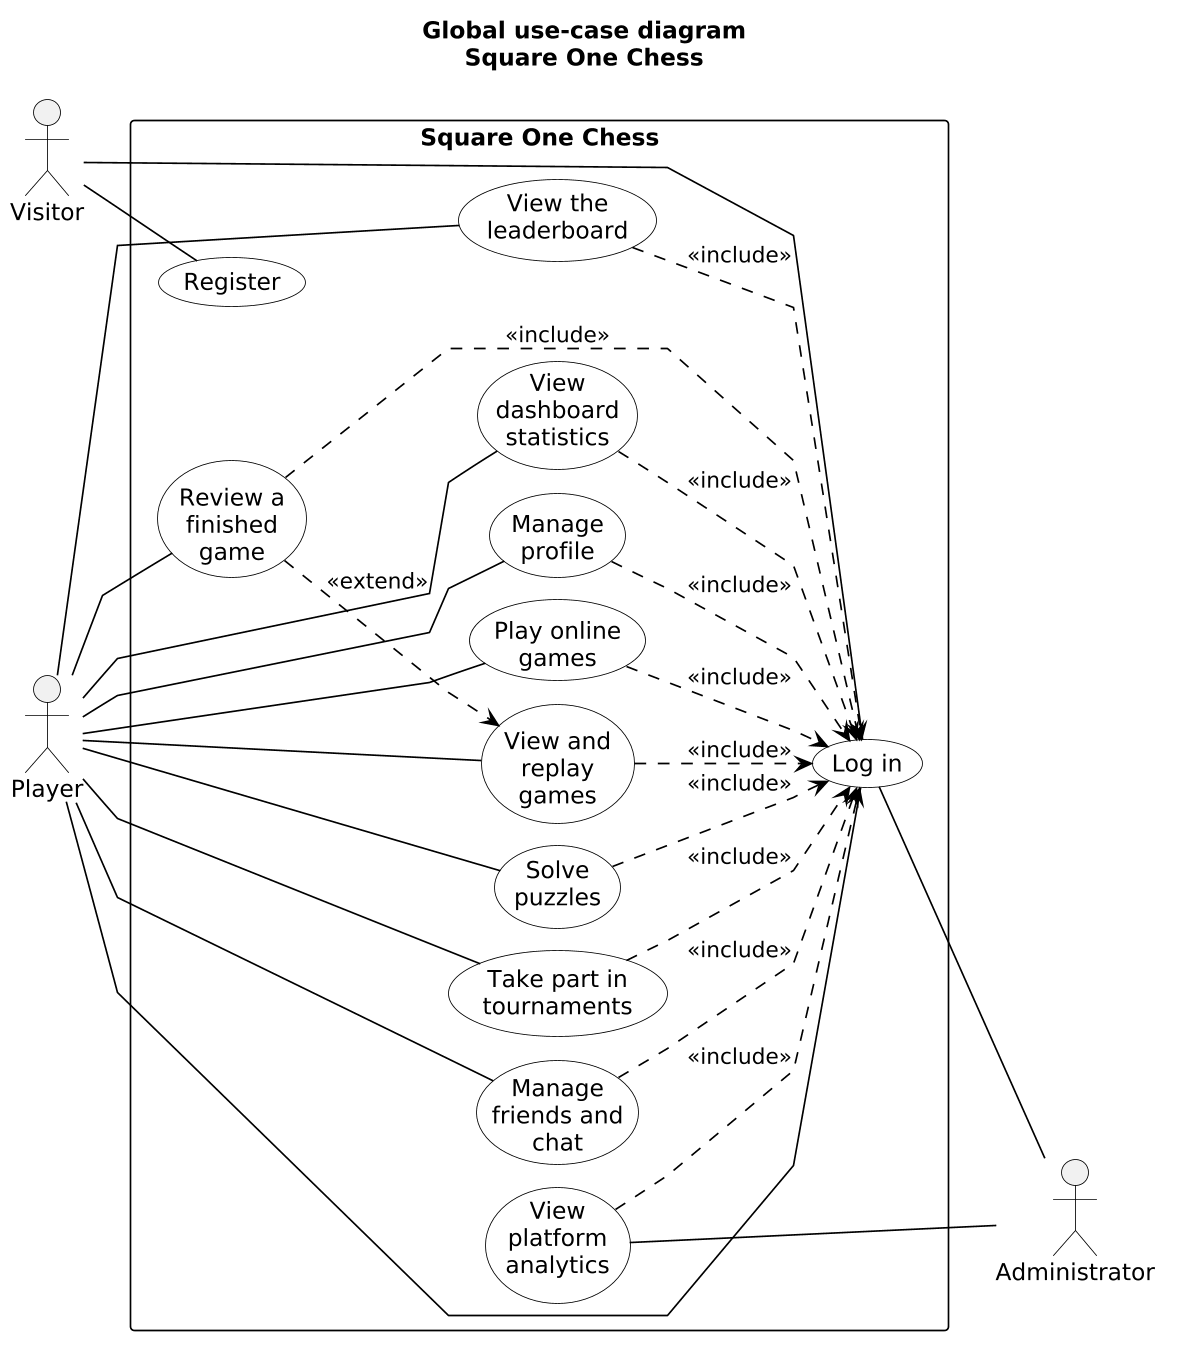
\includegraphics[width=\textwidth,height=0.80\textheight,keepaspectratio]{fig-usecase-global.png}%
}{\IfFileExists{uml/01-use-case.png}{%
  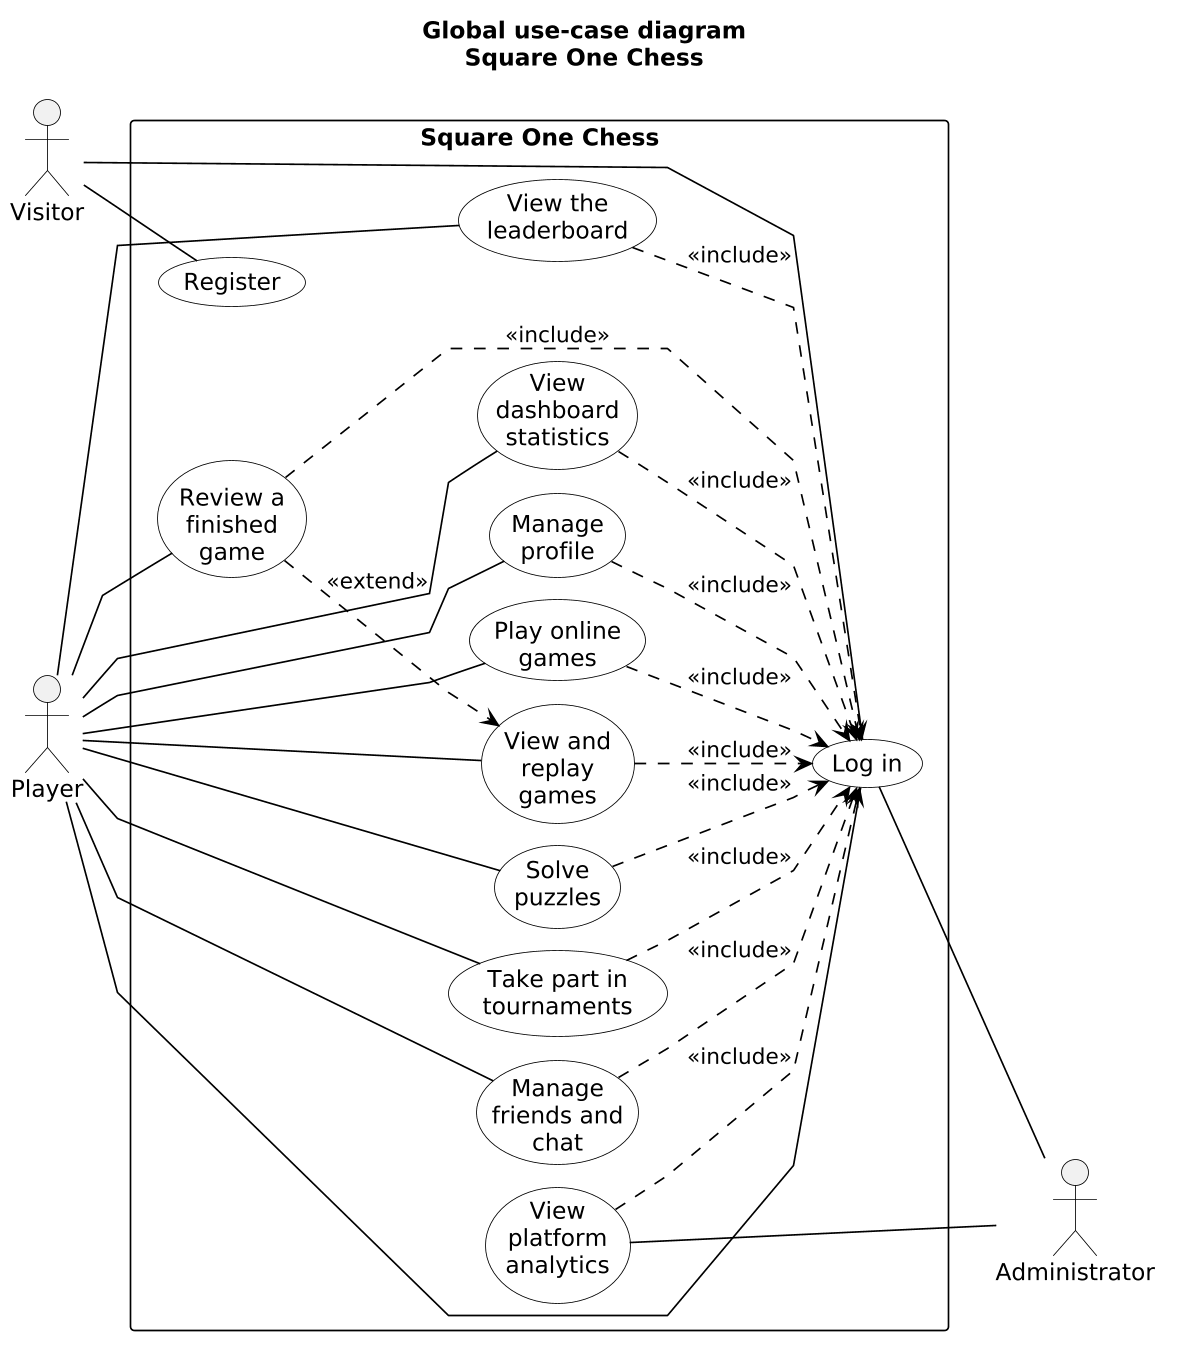
\includegraphics[width=\textwidth,height=0.80\textheight,keepaspectratio]{uml/01-use-case.png}%
}{\fbox{\parbox{0.88\linewidth}{\centering\vspace{8cm}\textit{[Upload fig-usecase-global.png]}\vspace{8cm}}}}}
\caption{Global use-case diagram}
\label{fig:uc-global}
\end{figure}
\clearpage

\section{Product backlog}
In order to ensure a clear and progressive organisation of the development, the product backlog was elaborated from the functional needs identified during the analysis phase.

{\small
\setlength{\tabcolsep}{4pt}
\renewcommand{\arraystretch}{1.28}
\begin{longtable}{|>{\raggedright\arraybackslash}p{0.46\linewidth}|c|c|c|c|}
\caption{Product backlog}
\label{tab:product-backlog}\\
\hline
\rowcolor{sectionblue}
\textcolor{white}{\textbf{User story}} &
\textcolor{white}{\textbf{Priority}} &
\textcolor{white}{\textbf{Estim.}} &
\textcolor{white}{\textbf{Sprint}} &
\textcolor{white}{\textbf{Release}} \\
\hline
\endfirsthead
\hline
\rowcolor{sectionblue}
\textcolor{white}{\textbf{User story}} &
\textcolor{white}{\textbf{Priority}} &
\textcolor{white}{\textbf{Estim.}} &
\textcolor{white}{\textbf{Sprint}} &
\textcolor{white}{\textbf{Release}} \\
\hline
\endhead
As a Visitor, I can register on the platform. & 1 & High & 1 & 1 \\
\hline
As a Player, I can log in and log out. & 1 & High & 2 & 1 \\
\hline
As a Player, I can manage my profile. & 1 & Medium & 2 & 1 \\
\hline
As a Player, I can play an online game with a clock. & 2 & High & 3 & 2 \\
\hline
As a Player, I can be paired automatically with an opponent. & 2 & High & 4 & 2 \\
\hline
As a Player, I can consult the history of my games. & 2 & Medium & 4 & 2 \\
\hline
As a Player, I can replay a finished game. & 2 & Medium & 4 & 2 \\
\hline
As a Player, I can manage friends and communicate. & 3 & High & 5 & 3 \\
\hline
As a Player, I can take part in tournaments. & 3 & Medium & 6 & 3 \\
\hline
As a Player, I can solve puzzles and train at chess. & 3 & Medium & 7 & 3 \\
\hline
As a Player, I can analyse a game with the AI review. & 3 & High & 7 & 3 \\
\hline
As a Player, I can consult the leaderboard and my statistics. & 3 & Medium & 8 & 3 \\
\hline
As an Administrator, I can supervise the activity of the platform. & 3 & Medium & 8 & 3 \\
\hline
\end{longtable}
}

\section{Conclusion}
In this chapter we presented the specification of the functional and non-functional requirements, as well as the different actors interacting with Square One. We also detailed the main features through the global use-case diagram and presented the product backlog. The next chapter is devoted to the first release of the project: access management and the account process.

\chapter{Release 1 --- Access and Accounts}
The first release of the project, entitled \textbf{Access and Accounts}, forms the functional and security foundation of Square One. It aims to put in place the essential mechanisms that control access to the application and to structure the registration path of new players.

\section{Sprint 1: Register}
\subsection{Introduction}
This first sprint was devoted to the fundamental features of the platform. The main objective was to allow a visitor to create a player account in a secure way, so that he can then access the services reserved to authenticated players.

\subsection{Sprint 1 backlog}
{\small
\renewcommand{\arraystretch}{1.3}
\setlength{\tabcolsep}{4pt}
\begin{table}[H]
\centering
\caption{Sprint 1 backlog}
\label{tab:sprint1-backlog}
\begin{tabularx}{\linewidth}{|>{\raggedright\arraybackslash}X|c|c|c|}
\hline
\rowcolor{sectionblue}
\textcolor{white}{\textbf{User story}} &
\textcolor{white}{\textbf{Priority}} &
\textcolor{white}{\textbf{Estim.}} &
\textcolor{white}{\textbf{Planning}} \\
\hline
As a Visitor, I can register on the platform. & 1 & High & Sprint 1 \\
\hline
As a Player, I can confirm my e-mail address. & 2 & Medium & Sprint 1 \\
\hline
\end{tabularx}
\end{table}
}

\subsection{Refinement of Sprint 1}
This sprint details the first contact of a visitor with Square One. The visitor creates an account (username, e-mail and password); the system stores the user and, when an e-mail service is configured, sends a confirmation message so that the address can be verified.

\paragraph{Refinement of the use case ``Register''.}
\umlfig{fig-uc-register.png}{Use-case diagram --- Register}

\begin{table}[H]
\centering
\caption{Refinement of the use case ``Register''}
\label{tab:uc-register}
\renewcommand{\arraystretch}{1.20}
\begin{tabularx}{\linewidth}{|>{\raggedright\bfseries}p{0.28\linewidth}|X|}
\hline
\rowcolor{sectionblue}
\multicolumn{2}{|c|}{\textcolor{white}{\textbf{Register}}} \\
\hline
Actor & Visitor. \\
\hline
Pre-condition & The system is running. The visitor is not authenticated. The visitor accesses the registration page. \\
\hline
Post-condition & A player account is created. The visitor is authenticated (JWT / HttpOnly cookie) and redirected to the e-mail verification page or to the dashboard. \\
\hline
Main scenario &
\begin{itemize}[leftmargin=1.1em,itemsep=0.15em,topsep=0.2em]
  \item The visitor opens the registration page.
  \item The system displays the registration form.
  \item The visitor enters a username, an e-mail address and a password.
  \item The visitor validates the form.
  \item The system checks the fields (e-mail format, password length, username).
  \item The system checks that the e-mail and the username are not already used.
  \item The system creates the account with a hashed password and initialises the profile (default Elo).
  \item The system generates a JWT and stores it in the cookie.
  \item The visitor accesses the services reserved to players.
\end{itemize} \\
\hline
Exception scenario &
If the data are invalid, if the e-mail already exists or if the username is already taken, the system displays an error message and no account is created. \\
\hline
\end{tabularx}
\end{table}

\subsection{Design of Sprint 1}
The design consists in specifying the system before its realisation. For the use case \textbf{Register}, we present the class diagram and the sequence diagram.

\paragraph{Design of the use case ``Register''.}
\noindent Diagram of classes:
\umlfig{fig-class-register.png}{Class diagram --- Register}

\noindent Sequence diagram:
\umlfig{fig-seq-register.png}{Sequence diagram --- Register}

\subsection{Realisation of Sprint 1}
The registration interface of Square One was designed to be simple and secure. The visitor enters a username, an e-mail address and a password. After validation, the API \texttt{POST /api/auth/register} creates the account, hashes the password and places an HttpOnly JWT cookie in the browser.

\uishot{ui-register.png}{Register interface}

\section{Sprint 2: Manage account}
\subsection{Introduction}
Sprint 2 focuses on the management of an existing account. The main objective is to allow a registered player to authenticate, to close his session, and to consult or update his profile (username) in a secure way.

\subsection{Sprint 2 backlog}
{\small
\renewcommand{\arraystretch}{1.3}
\setlength{\tabcolsep}{4pt}
\begin{table}[H]
\centering
\caption{Sprint 2 backlog}
\label{tab:sprint2-backlog}
\begin{tabularx}{\linewidth}{|>{\raggedright\arraybackslash}X|c|c|c|}
\hline
\rowcolor{sectionblue}
\textcolor{white}{\textbf{User story}} &
\textcolor{white}{\textbf{Priority}} &
\textcolor{white}{\textbf{Estim.}} &
\textcolor{white}{\textbf{Planning}} \\
\hline
As a Player, I can log in to the platform. & 1 & High & Sprint 2 \\
\hline
As a Player, I can log out. & 1 & High & Sprint 2 \\
\hline
As a Player, I can consult and edit my profile. & 2 & Medium & Sprint 2 \\
\hline
\end{tabularx}
\end{table}
}

\subsection{Refinement of Sprint 2}
This sprint covers the management of an existing account. The player logs in with his e-mail and password, can log out to close the session, and consults or updates his profile (username and displayed information).

\paragraph{Refinement of the use case ``Log in''.}
\umlfig{fig-uc-manage-account.png}{Use-case diagram --- Manage account}

\begin{table}[H]
\centering
\caption{Refinement of the use case ``Log in''}
\label{tab:uc-login}
\renewcommand{\arraystretch}{1.20}
\begin{tabularx}{\linewidth}{|>{\raggedright\bfseries}p{0.28\linewidth}|X|}
\hline
\rowcolor{sectionblue}
\multicolumn{2}{|c|}{\textcolor{white}{\textbf{Log in}}} \\
\hline
Actor & Player. \\
\hline
Pre-condition & The system is running. The player has a valid account. The player is not yet authenticated. \\
\hline
Post-condition & The player is authenticated. He is redirected to the lobby / dashboard. \\
\hline
Main scenario &
\begin{itemize}[leftmargin=1.1em,itemsep=0.15em,topsep=0.2em]
  \item The player opens the login page.
  \item The system displays the authentication form.
  \item The player enters his e-mail and his password.
  \item The player clicks on ``Log in''.
  \item The system checks the credentials (\texttt{POST /api/auth/login}).
  \item The system sets the HttpOnly JWT cookie and redirects the player.
\end{itemize} \\
\hline
Exception scenario &
If the password is wrong or the e-mail does not exist, the system displays an error message and no session is created. \\
\hline
\end{tabularx}
\end{table}

\begin{table}[H]
\centering
\caption{Refinement of the use case ``Manage profile''}
\label{tab:uc-profile}
\renewcommand{\arraystretch}{1.20}
\begin{tabularx}{\linewidth}{|>{\raggedright\bfseries}p{0.28\linewidth}|X|}
\hline
\rowcolor{sectionblue}
\multicolumn{2}{|c|}{\textcolor{white}{\textbf{Manage profile}}} \\
\hline
Actor & Player. \\
\hline
Pre-condition & The system is running. The player is authenticated. \\
\hline
Post-condition & The profile is displayed. If an update is submitted, the username is saved. \\
\hline
Main scenario &
\begin{itemize}[leftmargin=1.1em,itemsep=0.15em,topsep=0.2em]
  \item The player opens the profile page.
  \item The system loads the current user (\texttt{GET /api/auth/me}).
  \item The player clicks on ``Edit profile'', changes the username and validates.
  \item The system updates the account (\texttt{PUT /api/auth/profile}) and confirms.
\end{itemize} \\
\hline
Exception scenario &
If the new username is already taken, or if the session has expired, the system displays an error message and the profile is not modified. \\
\hline
\end{tabularx}
\end{table}

\subsection{Design of Sprint 2}
The design specifies the classes and the interactions for login and profile management before the realisation.

\paragraph{Design of the use case ``Log in'' / ``Manage profile''.}
\noindent Diagram of classes:
\umlfig{fig-class-login.png}{Class diagram --- Log in and manage profile}

\noindent Sequence diagram (log in):
\umlfig{fig-seq-login.png}{Sequence diagram --- Log in}

\noindent Sequence diagram (manage profile):
\umlfig{fig-seq-profile.png}{Sequence diagram --- Manage profile}

\subsection{Realisation of Sprint 2}
This section presents the implementation of the features developed during Sprint 2, devoted to authentication and to the player profile. After the registration of Sprint 1, this step completes the access path: login, logout and edition of the profile. The interfaces follow the same visual identity as the rest of the Angular client.

\paragraph{Login interface.}
The login page lets the player enter his e-mail and password. A successful request sets the session cookie; an error is shown when the credentials are invalid.

\uishot{ui-login.png}{Login interface}

\paragraph{Profile interface.}
The profile page displays the username, the Elo rating and the game statistics. The player can open the edit dialog to change his username.

\uishot{ui-profile.png}{Profile interface}

\section{Conclusion}
In this chapter we presented the first release of Square One, dedicated to access and accounts. Sprint 1 implemented the registration of a visitor. Sprint 2 completed the path with login, logout and profile management. The next chapter is devoted to Release 2: live play, matchmaking, history and replay.

\chapter{Release 2 --- Live Play}
The second release delivers the core of Square One: playing chess in real time. It covers the live board, the application of the rules, matchmaking, the history of games and replay.

\section{Sprint 3: Play online games}
\subsection{Introduction}
Sprint 3 implements a legal live game: clock, moves in real time, and a correct end of game (checkmate, resignation or draw). Play against the engine is included in this sprint.

\subsection{Sprint 3 backlog}
{\small
\renewcommand{\arraystretch}{1.3}
\setlength{\tabcolsep}{4pt}
\begin{table}[H]
\centering
\caption{Sprint 3 backlog}
\label{tab:sprint3-backlog}
\begin{tabularx}{\linewidth}{|>{\raggedright\arraybackslash}X|c|c|c|}
\hline
\rowcolor{sectionblue}
\textcolor{white}{\textbf{User story}} &
\textcolor{white}{\textbf{Priority}} &
\textcolor{white}{\textbf{Estim.}} &
\textcolor{white}{\textbf{Planning}} \\
\hline
As a Player, I can play an online game with a clock. & 1 & High & Sprint 3 \\
\hline
As a Player, I can send a legal move in real time. & 1 & High & Sprint 3 \\
\hline
As a Player, I can resign or offer a draw. & 2 & Medium & Sprint 3 \\
\hline
As a Player, I can play against the engine. & 2 & Medium & Sprint 3 \\
\hline
\end{tabularx}
\end{table}
}

\subsection{Refinement of Sprint 3}
This sprint specifies a legal live game: clocks, real-time moves, resignation and draw, and a correct end of game. The same board also lets the player face the engine (Stockfish) with a chosen difficulty.

\paragraph{Refinement of the use case ``Play online games''.}
\umlfig{fig-uc-play.png}{Use-case diagram --- Play online games}

\begin{table}[H]
\centering
\caption{Refinement of the use case ``Play online games''}
\label{tab:uc-play}
\renewcommand{\arraystretch}{1.20}
\begin{tabularx}{\linewidth}{|>{\raggedright\bfseries}p{0.28\linewidth}|X|}
\hline
\rowcolor{sectionblue}
\multicolumn{2}{|c|}{\textcolor{white}{\textbf{Play online games}}} \\
\hline
Actor & Player. \\
\hline
Pre-condition & The player is authenticated. A game exists (matchmaking or play versus the engine). \\
\hline
Post-condition & Each legal move is saved. When the game ends, the result and the PGN are stored. \\
\hline
Main scenario &
\begin{itemize}[leftmargin=1.1em,itemsep=0.15em,topsep=0.2em]
  \item The player opens the live board.
  \item The system shows the position (FEN) and the clock.
  \item The player plays a move.
  \item The system checks the move with \texttt{chess.js} and broadcasts it with Socket.io.
  \item The opponent's board is updated.
  \item On checkmate, resignation or draw, the game is closed.
\end{itemize} \\
\hline
Exception scenario &
If the move is illegal, if it is not the player's turn, or if the game is already finished, the system rejects the move. \\
\hline
\end{tabularx}
\end{table}

\subsection{Design of Sprint 3}
\paragraph{Design of the use case ``Play online games''.}
\noindent Diagram of classes:
\umlfig{fig-class-play.png}{Class diagram --- Play online games}

\noindent Sequence diagram:
\umlfig{fig-seq-move.png}{Sequence diagram --- Live move}

\subsection{Realisation of Sprint 3}
The game page shows the board, the clocks and the controls to resign or offer a draw. Moves travel through Socket.io; the server applies \texttt{chess.js} and stores each \texttt{Move}. Play versus the engine uses Stockfish with the chosen difficulty.

\uishot{ui-game.png}{Live game interface}

\section{Sprint 4: Matchmaking, history and replay}
\subsection{Introduction}
Sprint 4 adds pairing in the lobby, the list of past games, and the replay of a finished game.

\subsection{Sprint 4 backlog}
{\small
\renewcommand{\arraystretch}{1.3}
\setlength{\tabcolsep}{4pt}
\begin{table}[H]
\centering
\caption{Sprint 4 backlog}
\label{tab:sprint4-backlog}
\begin{tabularx}{\linewidth}{|>{\raggedright\arraybackslash}X|c|c|c|}
\hline
\rowcolor{sectionblue}
\textcolor{white}{\textbf{User story}} &
\textcolor{white}{\textbf{Priority}} &
\textcolor{white}{\textbf{Estim.}} &
\textcolor{white}{\textbf{Planning}} \\
\hline
As a Player, I can join matchmaking. & 1 & High & Sprint 4 \\
\hline
As a Player, I can consult my game history. & 1 & Medium & Sprint 4 \\
\hline
As a Player, I can replay a finished game. & 2 & Medium & Sprint 4 \\
\hline
\end{tabularx}
\end{table}
}

\subsection{Refinement of Sprint 4}
This sprint describes how a player is paired with an opponent of similar Elo, then how he consults his finished games and replays the moves stored for a selected match.

\paragraph{Refinement of the use cases ``Join matchmaking'' and ``Consult and replay games''.}
\umlfig{fig-uc-match-history.png}{Use-case diagram --- Matchmaking, history and replay}

\begin{table}[H]
\centering
\caption{Refinement of the use case ``Join matchmaking''}
\label{tab:uc-match}
\renewcommand{\arraystretch}{1.20}
\begin{tabularx}{\linewidth}{|>{\raggedright\bfseries}p{0.28\linewidth}|X|}
\hline
\rowcolor{sectionblue}
\multicolumn{2}{|c|}{\textcolor{white}{\textbf{Join matchmaking}}} \\
\hline
Actor & Player. \\
\hline
Pre-condition & The player is authenticated and is not already in a live game. \\
\hline
Post-condition & Two players are paired. A \texttt{Game} is created and both clients open the board. \\
\hline
Main scenario &
\begin{itemize}[leftmargin=1.1em,itemsep=0.15em,topsep=0.2em]
  \item The player chooses a time control and joins the queue.
  \item The system stores a \texttt{QueueEntry} (user, Elo).
  \item When a suitable opponent is found, the system creates the game and notifies both players.
\end{itemize} \\
\hline
Exception scenario &
If the player leaves the queue, the entry is removed. If no opponent is available, the player waits. \\
\hline
\end{tabularx}
\end{table}

\begin{table}[H]
\centering
\caption{Refinement of the use case ``Consult and replay games''}
\label{tab:uc-replay}
\renewcommand{\arraystretch}{1.20}
\begin{tabularx}{\linewidth}{|>{\raggedright\bfseries}p{0.28\linewidth}|X|}
\hline
\rowcolor{sectionblue}
\multicolumn{2}{|c|}{\textcolor{white}{\textbf{Consult and replay games}}} \\
\hline
Actor & Player. \\
\hline
Pre-condition & The player is authenticated. At least one finished game exists. \\
\hline
Post-condition & The list of games is displayed. In replay, the player can step through the moves. \\
\hline
Main scenario &
\begin{itemize}[leftmargin=1.1em,itemsep=0.15em,topsep=0.2em]
  \item The player opens the history.
  \item The system returns his games (result, time control, PGN).
  \item The player selects a game and replays the moves one by one.
\end{itemize} \\
\hline
Exception scenario &
If the list is empty, the system shows an empty state. If the game cannot be loaded, an error is displayed. \\
\hline
\end{tabularx}
\end{table}

\subsection{Design of Sprint 4}
\paragraph{Design of matchmaking, history and replay.}
\noindent Diagram of classes:
\umlfig{fig-class-match.png}{Class diagram --- Matchmaking, history and replay}

\noindent Sequence diagram (matchmaking):
\umlfig{fig-seq-match.png}{Sequence diagram --- Matchmaking}

\noindent Sequence diagram (replay):
\umlfig{fig-seq-replay.png}{Sequence diagram --- Replay}

\subsection{Realisation of Sprint 4}
The lobby lets the player join a queue and wait for a match. The history lists finished games. Replay walks through the stored moves / PGN.

\uishot{ui-lobby.png}{Lobby / matchmaking}
\uishot{ui-history.png}{Game history and replay}

\section{Conclusion}
Release 2 added live play (Sprint 3) and pairing, history and replay (Sprint 4). The next chapter covers the community, training and supervision of the platform.

\chapter{Release 3 --- Community, Training and Supervision}
The third release completes Square One with a community layer, structured competitions, training tools and a supervision space for the administrator.

\section{Sprint 5: Communicate with players}
\subsection{Introduction}
Sprint 5 adds friends and in-game chat: a player can send or accept a friend request, see who is online, and exchange messages during a live game.

\subsection{Sprint 5 backlog}
{\small
\renewcommand{\arraystretch}{1.3}
\begin{table}[H]
\centering
\caption{Sprint 5 backlog}
\label{tab:sprint5-backlog}
\begin{tabularx}{\linewidth}{|>{\raggedright\arraybackslash}X|c|c|c|}
\hline
\rowcolor{sectionblue}
\textcolor{white}{\textbf{User story}} &
\textcolor{white}{\textbf{Priority}} &
\textcolor{white}{\textbf{Estim.}} &
\textcolor{white}{\textbf{Planning}} \\
\hline
As a Player, I can manage my friends. & 1 & High & Sprint 5 \\
\hline
As a Player, I can chat with other players. & 1 & High & Sprint 5 \\
\hline
As a Player, I can see who is online. & 2 & Medium & Sprint 5 \\
\hline
\end{tabularx}
\end{table}
}

\subsection{Refinement of Sprint 5}
This sprint describes the community layer. A player sends or accepts a friend request, sees who is online, and exchanges messages in the chat of the current game.

\paragraph{Refinement of the use case ``Communicate with players''.}
\umlfig{fig-uc-social.png}{Use-case diagram --- Communicate with players}

\begin{table}[H]
\centering
\caption{Refinement of the use case ``Communicate with players''}
\label{tab:uc-social}
\renewcommand{\arraystretch}{1.20}
\begin{tabularx}{\linewidth}{|>{\raggedright\bfseries}p{0.28\linewidth}|X|}
\hline
\rowcolor{sectionblue}
\multicolumn{2}{|c|}{\textcolor{white}{\textbf{Communicate with players}}} \\
\hline
Actor & Player. \\
\hline
Pre-condition & The player is authenticated. \\
\hline
Post-condition & Friend links and messages are stored. \\
\hline
Main scenario &
\begin{itemize}[leftmargin=1.1em,itemsep=0.15em,topsep=0.2em]
  \item The player sends or accepts a friend request.
  \item The system updates the \texttt{Friend} status.
  \item The player sends a message in the chat of the current game.
  \item Socket.io delivers the \texttt{GameMessage} to the two players of that game.
\end{itemize} \\
\hline
Exception scenario &
If the request already exists or the session expired, the system shows an error. \\
\hline
\end{tabularx}
\end{table}

\subsection{Design of Sprint 5}
The design specifies the classes and the interactions for friends and chat before the realisation.

\paragraph{Design of the use case ``Communicate with players''.}
\noindent Diagram of classes:
\umlfig{fig-class-social.png}{Class diagram --- Communicate with players}

\noindent Sequence diagram (in-game chat):
\umlfig{fig-seq-chat.png}{Sequence diagram --- In-game chat}

\subsection{Realisation of Sprint 5}
This section presents the implementation of the features developed during Sprint 5. After the live game of Release 2, this step adds a community layer: friend requests and real-time messages.

\paragraph{Friends and chat interface.}
The player can send or accept a friend request and see who is connected. During a live game, the in-game chat sends a \texttt{GameMessage} through Socket.io to the room \texttt{game:\{gameId\}}. Presence follows the socket session.

\uishot{ui-friends-chat.png}{Friends and chat}

\section{Sprint 6: Tournaments}
\subsection{Introduction}
Sprint 6 lets a player create or join a tournament and follow the bracket and the matches.

\subsection{Sprint 6 backlog}
{\small
\renewcommand{\arraystretch}{1.3}
\begin{table}[H]
\centering
\caption{Sprint 6 backlog}
\label{tab:sprint6-backlog}
\begin{tabularx}{\linewidth}{|>{\raggedright\arraybackslash}X|c|c|c|}
\hline
\rowcolor{sectionblue}
\textcolor{white}{\textbf{User story}} &
\textcolor{white}{\textbf{Priority}} &
\textcolor{white}{\textbf{Estim.}} &
\textcolor{white}{\textbf{Planning}} \\
\hline
As a Player, I can create or join a tournament. & 1 & High & Sprint 6 \\
\hline
As a Player, I can follow the bracket and the matches. & 2 & Medium & Sprint 6 \\
\hline
\end{tabularx}
\end{table}
}

\subsection{Refinement of Sprint 6}
This sprint specifies structured competitions. A player creates a tournament or joins an open one; the system records the registration and displays the bracket of the rounds and the linked matches.

\paragraph{Refinement of the use case ``Take part in tournaments''.}
\umlfig{fig-uc-tournament.png}{Use-case diagram --- Take part in tournaments}

\begin{table}[H]
\centering
\caption{Refinement of the use case ``Take part in tournaments''}
\label{tab:uc-tournament}
\renewcommand{\arraystretch}{1.20}
\begin{tabularx}{\linewidth}{|>{\raggedright\bfseries}p{0.28\linewidth}|X|}
\hline
\rowcolor{sectionblue}
\multicolumn{2}{|c|}{\textcolor{white}{\textbf{Take part in tournaments}}} \\
\hline
Actor & Player. \\
\hline
Pre-condition & The player is authenticated. The tournament is open. \\
\hline
Post-condition & A \texttt{TournamentRegistration} is created. Matches appear in the bracket. \\
\hline
Main scenario &
\begin{itemize}[leftmargin=1.1em,itemsep=0.15em,topsep=0.2em]
  \item The player opens the tournament page.
  \item He creates a tournament or joins an existing one.
  \item The system records the registration and shows the bracket.
\end{itemize} \\
\hline
Exception scenario &
If the tournament is full or the player is already registered, the join is refused. \\
\hline
\end{tabularx}
\end{table}

\subsection{Design of Sprint 6}
The design specifies the tournament entities and the join sequence before the realisation.

\paragraph{Design of the use case ``Take part in tournaments''.}
\noindent Diagram of classes:
\umlfig{fig-class-tournament.png}{Class diagram --- Tournaments}

\noindent Sequence diagram (join):
\umlfig{fig-seq-tournament.png}{Sequence diagram --- Join a tournament}

\subsection{Realisation of Sprint 6}
This section presents the implementation of tournaments. A player creates an event or joins an open one; the server stores a \texttt{TournamentRegistration} and builds the bracket (\texttt{TournamentMatch} linked to a \texttt{Game}).

\paragraph{Tournament interface.}
The tournament page lists open events, the registered players and the bracket of the rounds.

\uishot{ui-tournament.png}{Tournament page}

\section{Sprint 7: Train at chess}
\subsection{Introduction}
Sprint 7 adds tactical puzzles and the AI review of a finished game (Stockfish / analysis API). Play versus the engine was already delivered in Sprint 3.

\subsection{Sprint 7 backlog}
{\small
\renewcommand{\arraystretch}{1.3}
\begin{table}[H]
\centering
\caption{Sprint 7 backlog}
\label{tab:sprint7-backlog}
\begin{tabularx}{\linewidth}{|>{\raggedright\arraybackslash}X|c|c|c|}
\hline
\rowcolor{sectionblue}
\textcolor{white}{\textbf{User story}} &
\textcolor{white}{\textbf{Priority}} &
\textcolor{white}{\textbf{Estim.}} &
\textcolor{white}{\textbf{Planning}} \\
\hline
As a Player, I can solve puzzles. & 1 & High & Sprint 7 \\
\hline
As a Player, I can analyse a game (AI review). & 2 & Medium & Sprint 7 \\
\hline
\end{tabularx}
\end{table}
}

\subsection{Refinement of Sprint 7}
This sprint covers training besides live play. The player solves tactical puzzles from a FEN position; he can also request an AI review of a finished game, based on the analysis API and Stockfish.

\paragraph{Refinement of the use case ``Train at chess''.}
\umlfig{fig-uc-train.png}{Use-case diagram --- Train at chess}

\begin{table}[H]
\centering
\caption{Refinement of the use case ``Train at chess''}
\label{tab:uc-train}
\renewcommand{\arraystretch}{1.20}
\begin{tabularx}{\linewidth}{|>{\raggedright\bfseries}p{0.28\linewidth}|X|}
\hline
\rowcolor{sectionblue}
\multicolumn{2}{|c|}{\textcolor{white}{\textbf{Train at chess}}} \\
\hline
Actor & Player. \\
\hline
Pre-condition & The player is authenticated. Puzzles exist in the database. \\
\hline
Post-condition & Attempts and solves are stored in \texttt{UserPuzzleStats}. A review can be displayed for a finished game. \\
\hline
Main scenario &
\begin{itemize}[leftmargin=1.1em,itemsep=0.15em,topsep=0.2em]
  \item The player opens the puzzle page.
  \item The system returns a public puzzle DTO (FEN, theme, rating, number of plies) without revealing the solution line.
  \item The player plays move by move; each correct ply may auto-play the opponent reply until the line is finished and recorded in \texttt{UserPuzzleStats}.
  \item Optionally he asks for a hint (piece square) or an AI review of a past game (\texttt{/api/ai}).
\end{itemize} \\
\hline
Exception scenario &
If no puzzle is available, the move is wrong, or the review fails, the system shows an error or resets the board. \\
\hline
\end{tabularx}
\end{table}

\subsection{Design of Sprint 7}
The design specifies the puzzle model and the solve sequence before the realisation.

\paragraph{Design of the use case ``Train at chess''.}
\noindent Diagram of classes:
\umlfig{fig-class-train.png}{Class diagram --- Training}

\noindent Sequence diagram (puzzle):
\umlfig{fig-seq-puzzle.png}{Sequence diagram --- Solve a puzzle}

\subsection{Realisation of Sprint 7}
This section presents the training tools. Play versus the engine was already delivered in Sprint 3; Sprint 7 adds tactical puzzles and the AI review of a finished game.

\paragraph{Puzzle and review interface.}
The puzzle page shows a FEN position (daily, random or filtered by theme). Solving is multi-ply: a correct move can trigger the stored opponent reply, then the next player ply, until the line ends. Attempts and successes are stored in \texttt{UserPuzzleStats}. The review of a past game calls \texttt{/api/ai}, backed by Stockfish.

\uishot{ui-puzzles.png}{Puzzle and review}

\section{Sprint 8: Analyse performance and administer}
\subsection{Introduction}
Sprint 8 exposes the leaderboard and personal statistics to the player, and an analytics view to the administrator.

\subsection{Sprint 8 backlog}
{\small
\renewcommand{\arraystretch}{1.3}
\begin{table}[H]
\centering
\caption{Sprint 8 backlog}
\label{tab:sprint8-backlog}
\begin{tabularx}{\linewidth}{|>{\raggedright\arraybackslash}X|c|c|c|}
\hline
\rowcolor{sectionblue}
\textcolor{white}{\textbf{User story}} &
\textcolor{white}{\textbf{Priority}} &
\textcolor{white}{\textbf{Estim.}} &
\textcolor{white}{\textbf{Planning}} \\
\hline
As a Player, I can consult the leaderboard and my statistics. & 1 & High & Sprint 8 \\
\hline
As an Administrator, I can supervise the activity of the platform. & 2 & Medium & Sprint 8 \\
\hline
\end{tabularx}
\end{table}
}

\subsection{Refinement of Sprint 8}
This sprint distinguishes two views of the same data. The player consults the leaderboard and his personal statistics; the administrator opens an analytics page that summarises the activity of the platform, without modifying any game.

\paragraph{Refinement of the use cases ``Analyse performance'' and ``Administer the platform''.}
\umlfig{fig-uc-stats-admin.png}{Use-case diagram --- Statistics and administration}

\begin{table}[H]
\centering
\caption{Refinement of the use case ``Analyse performance''}
\label{tab:uc-stats}
\renewcommand{\arraystretch}{1.20}
\begin{tabularx}{\linewidth}{|>{\raggedright\bfseries}p{0.28\linewidth}|X|}
\hline
\rowcolor{sectionblue}
\multicolumn{2}{|c|}{\textcolor{white}{\textbf{Analyse performance}}} \\
\hline
Actor & Player. \\
\hline
Pre-condition & The player is authenticated. \\
\hline
Post-condition & The leaderboard and the personal statistics are displayed. \\
\hline
Main scenario &
\begin{itemize}[leftmargin=1.1em,itemsep=0.15em,topsep=0.2em]
  \item The player opens the leaderboard (\texttt{GET /api/stats}).
  \item The system orders users by Elo.
  \item The player can also consult his own counters (games played and won).
\end{itemize} \\
\hline
Exception scenario &
If the session has expired, the system redirects to the login page. \\
\hline
\end{tabularx}
\end{table}

\begin{table}[H]
\centering
\caption{Refinement of the use case ``Administer the platform''}
\label{tab:uc-admin}
\renewcommand{\arraystretch}{1.20}
\begin{tabularx}{\linewidth}{|>{\raggedright\bfseries}p{0.28\linewidth}|X|}
\hline
\rowcolor{sectionblue}
\multicolumn{2}{|c|}{\textcolor{white}{\textbf{Administer the platform}}} \\
\hline
Actor & Administrator. \\
\hline
Pre-condition & The user is authenticated with the supervision right. \\
\hline
Post-condition & KPIs are displayed. No game data are modified. \\
\hline
Main scenario &
\begin{itemize}[leftmargin=1.1em,itemsep=0.15em,topsep=0.2em]
  \item The administrator opens the analytics page.
  \item The system returns an overview (\texttt{/api/analytics}): users, games and activity.
\end{itemize} \\
\hline
Exception scenario &
If the user is not allowed, the API returns 403. \\
\hline
\end{tabularx}
\end{table}

\subsection{Design of Sprint 8}
The design specifies the statistics services and the leaderboard sequence before the realisation.

\paragraph{Design of statistics and administration.}
\noindent Diagram of classes:
\umlfig{fig-class-stats.png}{Class diagram --- Statistics and administration}

\noindent Sequence diagram (leaderboard):
\umlfig{fig-seq-leaderboard.png}{Sequence diagram --- Leaderboard}

\subsection{Realisation of Sprint 8}
This section presents the ranking for the player and the supervision view for the administrator. Rankings use the Elo and the game counters stored on \texttt{User}. Analytics aggregates users and games without modifying any game data.

\paragraph{Leaderboard interface.}
The leaderboard lists players ordered by Elo. The profile also shows personal statistics (games played and won).

\uishot{ui-leaderboard.png}{Leaderboard}

\paragraph{Analytics interface.}
The analytics page is reserved to the administrator (\texttt{/api/analytics}). An unauthorised request is rejected with 403.

\uishot{ui-analytics.png}{Analytics dashboard}

\section{Conclusion}
Release 3 added friends and chat, tournaments, puzzles and AI review, then statistics and administration. This completes the functional scope of Square One described in the product backlog.

\chapter*{General Conclusion}
\addcontentsline{toc}{chapter}{General Conclusion}

At the end of this project, we designed and developed a complete real-time chess web platform named \textbf{Square One}, answering the functional and organisational needs identified during the preliminary study.

The application integrates several essential features for the different actors of the system. A visitor can create an account and log in. A player can manage his profile, join matchmaking or play against the engine, follow a live game with a clock, consult his history, replay a finished game, solve puzzles, open an AI review, take part in tournaments, manage friends and chat, and consult the leaderboard as well as his dashboard statistics. The administrator can supervise the platform through a global analytics view.

Advanced features such as real-time play with Socket.io, the social sidebar (friends and chat), tournaments with a bracket, tactical puzzles and the Stockfish analysis of finished games give Square One a clear added value compared with a simple static chess page.

The project was structured according to an Agile Scrum approach, organised into three releases and eight progressive sprints. The use of modern technologies such as Angular~17, Node.js, Express, Prisma, SQLite, Socket.io, chess.js and Stockfish made it possible to obtain a clear, structured and maintainable design.

Despite the results obtained, some aspects still present limits. The interface can still be improved on certain screens. Play against the engine remains limited to a few difficulty levels. There is no spectator mode for ongoing games, and the internship did not include a production deployment of the platform.

Among the future perspectives, we can mention:
\begin{itemize}[leftmargin=1.4em]
  \item The addition of a spectator mode for live games.
  \item Finer engine levels and a richer analysis of games.
  \item The development of a mobile application.
  \item A production deployment with a more robust hosting of the API and the database.
  \item A richer ranking and more detailed statistics for the player and the administrator.
\end{itemize}

This project allowed us to consolidate our technical skills in full-stack web development, UML design and agile project management. Square One thus constitutes a solid base for an evolvable solution, able to answer the current and future needs of an online chess community.

\chapter*{Webography}
\addcontentsline{toc}{chapter}{Webography}

\begin{itemize}[leftmargin=2.6em,label={},itemsep=0.45em]
  \webitem{1}{angular}{Angular documentation}{https://angular.dev}{12/09/2026}
  \webitem{2}{html5}{HTML5}{https://developer.mozilla.org/en-US/docs/Web/HTML}{12/09/2026}
  \webitem{3}{css3}{CSS3}{https://developer.mozilla.org/en-US/docs/Web/CSS}{12/09/2026}
  \webitem{4}{tailwind}{Tailwind CSS}{https://tailwindcss.com}{13/09/2026}
  \webitem{5}{javascript}{JavaScript}{https://developer.mozilla.org/en-US/docs/Web/JavaScript}{13/09/2026}
  \webitem{6}{typescript}{TypeScript}{https://www.typescriptlang.org}{13/09/2026}
  \webitem{7}{nodejs}{Node.js}{https://nodejs.org}{14/09/2026}
  \webitem{8}{express}{Express.js}{https://expressjs.com}{14/09/2026}
  \webitem{9}{prisma}{Prisma}{https://www.prisma.io}{14/09/2026}
  \webitem{10}{sqlite}{SQLite}{https://www.sqlite.org}{15/09/2026}
  \webitem{11}{socketio}{Socket.io}{https://socket.io}{15/09/2026}
  \webitem{12}{chessjs}{chess.js}{https://github.com/jhlywa/chess.js}{15/09/2026}
  \webitem{13}{stockfish}{Stockfish}{https://stockfishchess.org}{16/09/2026}
  \webitem{14}{vscode}{Visual Studio Code}{https://code.visualstudio.com}{16/09/2026}
  \webitem{15}{git}{Git}{https://git-scm.com}{16/09/2026}
  \webitem{16}{github}{GitHub}{https://github.com}{17/09/2026}
  \webitem{17}{postman}{Postman}{https://www.postman.com}{17/09/2026}
  \webitem{18}{plantuml}{PlantUML}{https://plantuml.com}{17/09/2026}
\end{itemize}

\end{document}
